\documentclass[a4paper,14pt]{extreport} %размер бумаги устанавливаем А4, шрифт 14пунктов
\usepackage[T2A]{fontenc}
\usepackage[utf8]{inputenc} 
\usepackage[english,russian]{babel}
\usepackage{amssymb,amsfonts,amsmath,cite,enumerate,float} % подключаем нужные пакеты расширений
\usepackage{graphicx} % хотим вставлять в диплом рисунки
\usepackage{longtable} % для таблиц длиннее, чем на страницу
\usepackage{misccorr} % Добавляем "точки" после названий разделов
\usepackage{geometry} % Меняем поля страницы
\usepackage{indentfirst}%отступ первого абзаца после названия главы
\usepackage{setspace}
\usepackage{fancyhdr} 
\usepackage {titlesec} % название главы по центру


\graphicspath{{images/}}



\makeatletter
\renewcommand{\@biblabel}[1]{#1.} % Заменяем библиографию с квадратных скобок на точку
\makeatother

\geometry{left=2.5cm}% левое поле
\geometry{right=2cm}% правое поле
\geometry{top=2cm}% верхнее поле
\geometry{bottom=2cm}% нижнее поле

\setcounter{secnumdepth}{4}% уровень вложенности счётчиков

\onehalfspacing

\titleformat{\chapter}{\thispagestyle{myheadings}\centering\hyphenpenalty=10000\normalfont\huge\bfseries}{
\thechapter. }{0pt}{\Huge}
\makeatother
\setlength{\headheight}{17pt}

%нумерация справа вверху
\pagestyle{fancy} 
\lhead{} \chead{} \rhead{\normalsize\thepage}
\lfoot{} \cfoot{} \rfoot{}
\renewcommand{\headrulewidth}{0pt}
\renewcommand{\footrulewidth}{0pt}
\fancypagestyle{plain}{%
    \fancyhf{} % clear all header and footer fields
    \fancyhead[RE,RO]{\normalsize \thepage} % Even page, Odd page; Right, Left, Center
    \renewcommand{\headrulewidth}{0pt}
    \renewcommand{\footrulewidth}{0pt}
}

% для большой таблицы
\newenvironment{myTable}{%
    \tiny
    \begin{longtable}[H]{|p{0.9cm}|p{3.4cm}|p{1.2cm}|p{3.9cm}|p{0.6cm}|p{0.7cm}|p{0.6cm}|p{0.7cm}|}
    \hline
}{
    \end{longtable}
}

% для большой таблицы
\newenvironment{myTableSecond}{
    \scriptsize
    \begin{longtable}[H]{|p{0.7cm}|p{0.4cm}|p{0.4cm}|p{0.9cm}|p{0.9cm}|p{0.9cm}|p{0.9cm}|p{0.9cm}|p{0.9cm}|p{0.9cm}|}
	\caption{Параметры сетевой модели}\\
	\label{psm}
    \hline
}{
    \end{longtable}
}


%перечисления
%\renewcommand{\theenumi}{\arabic{enumi}}% Меняем везде перечисления на цифра.цифра
%\renewcommand{\labelenumi}{\arabic{enumi}}% Меняем везде перечисления на цифра.цифра
%\renewcommand{\theenumii}{.\arabic{enumii}}% Меняем везде перечисления на цифра.цифра
%\renewcommand{\labelenumii}{\arabic{enumi}.\arabic{enumii}.}% Меняем везде перечисления на цифра.цифра
%\renewcommand{\theenumiii}{.\arabic{enumiii}}% Меняем везде перечисления на цифра.цифра
%\renewcommand{\labelenumiii}{\arabic{enumi}.\arabic{enumii}.\arabic{enumiii}}% Меняем везде перечисления на цифра.цифра

%полуторный интервал между строками
%\renewcommand{\baselinestretch}{1.5}% вроде как плохой метод, т.к. растягивает заголовки и сноски, чего лучше не делать


\renewcommand{\contentsname}{Содержание} 
\setcounter{page}{2}


\setlength{\parindent}{1cm}

\begin{document}


\title{Программно"=аппаратный комплекс для~создания диалоговых когнитивных роботов на~основе реактивно"=делиберативного подхода}
\author{oserikov}
\maketitle% это титульный лист
\chapter*{РЕФЕРАТ}
Выпускная квалификационная работа содержит: \pageref{LastPage}\ страниц, \totalfigures\ рисунков, 2 источника.

ИСКУССТВЕННЫЙ ИНТЕЛЛЕКТ, КОГНИТИВНЫЕ ТЕХНОЛОГИИ, ДИАЛОГОВЫЕ СИСТЕМЫ, РЕАКТИВНЫЙ ПОДХОД, ДЕЛИБЕРАТИВНЫЙ ПОДХОД, ОБЛАЧНЫЕ ТЕХНОЛОГИИ, MICROSOFT AZURE, ИНТЕРНЕТ ВЕЩЕЙ, NOSQL.

В данной работе поставлена и решена задача создания программно"=аппаратного комплекса для создания диалоговых когнитивных роботов на~основе реактивно"=делиберативного подхода.

В теоретической части работы приведены рассуждения, предшествующие постановке задачи, оценена актуальность задачи и исследованы предпосылки к постановке задачи.

В практической части работы описан разработанный подход к решению задачи с использованием реактивно"=делиберативного подхода, поддерживаемого облачными технологиями. Рассмотрены ключевые элементы как аппаратной части решения, так и программной части.
\pagebreak
\tableofcontents
\prettypart{ВВЕДЕНИЕ}

В настоящее время возросшая скорость жизни как в её частных деталях, так и в общем, вынуждает человечество автоматизировать всё, что кажется возможным автоматизировать. Автоматизации подвергается как механическая деятельность человека --- промышленная революция, например ---, так и (особенно в последнее время вследствие общего увеличения доступных вычислительных мощностей) когнитивная деятельность человека.

Одной из идей, лежащих в основе механической автоматизации, является идея о создании роботов, выполняющих те или иные механические задачи.

Одной из идей, лежащих в основе когнитивной автоматизации, является идея об искусственном интеллекте, выполняющем те или иные интеллектуальные задачи.

Одной из задач, активно автоматизируемых в наши дни, является задача реализации образовательного процесса.

\chapter*{Рассуждения, приводящие к постановке\\ задачи ВКР}
Задача, сформулированная и решённая в выпускной квалификационной работе, поставлена на стыке нескольких технологически"=социальных явлений.

\section*{Доступная робототехника}
Развитию робототехники и, следовательно, образовательной робототехники значительно способствует снижение стоимости робототехнических решений начального уровня. В последние годы появилось большое количество микроконтроллеров и одноплатных компьютеров, позволяющих приобщиться к робототехнике большинству заинтересованных.

Набирает обороты движение <<мейкеров>>, использующих подручные и доступные средства для решения бытовых задач, творчества и развлечения на основе инженерного подхода.

% \subsection*{Популярные инструменты}
\label{popular-instruments}
Среди доступных элементов робототехники особенно заметны два класса устройств: микроконтроллеры и микрокомпьютеры.

Среди микроконтроллеров самыми популярными являются устройства семейства Arduino.

Среди микрокомпьютеров самыми популярными являются устройства семейства Raspberry Pi.

Оба семейства продуктов существуют достаточно долго, что привело к формированию сплочённого сообщества специалистов, что значительно снижает порог начала использования устройств: большая часть задач, интересных новичку, решена и разобрана в виде обучающего материала кем"=то в сети интернет.

\section*{Образовательная робототехника}
Образовательные технологии, как источник и следствие научного прогресса, находятся в постоянном развитии, постоянно влияя на общество. Текущее состояние образовательных технологий, направление их развития --- это наглядная демонстрация состояния и развития как общества, так и науки в наши дни.

% https://books.google.com/ngrams/graph?content=educational+robotics&case_insensitive=on&year_start=1980&year_end=2008&corpus=15&smoothing=3&share=&direct_url=t4%3B%2Ceducational%20robotics%3B%2Cc0%3B%2Cs0%3B%3Beducational%20robotics%3B%2Cc0%3B%3BEducational%20Robotics%3B%2Cc0
Сегодня одним из набирающих популярность направлений развития образовательных технологий является образовательная робототехника, что подтверждается исследованием корпусов Google Books English средствами Google Ngram \cite{google-ngram} по запросу $[\texttt{educational\ robotics}]$.


\begin{figure}[H]
\renewcommand\thefigure{0.1} % Make this Figure A
    \centering
    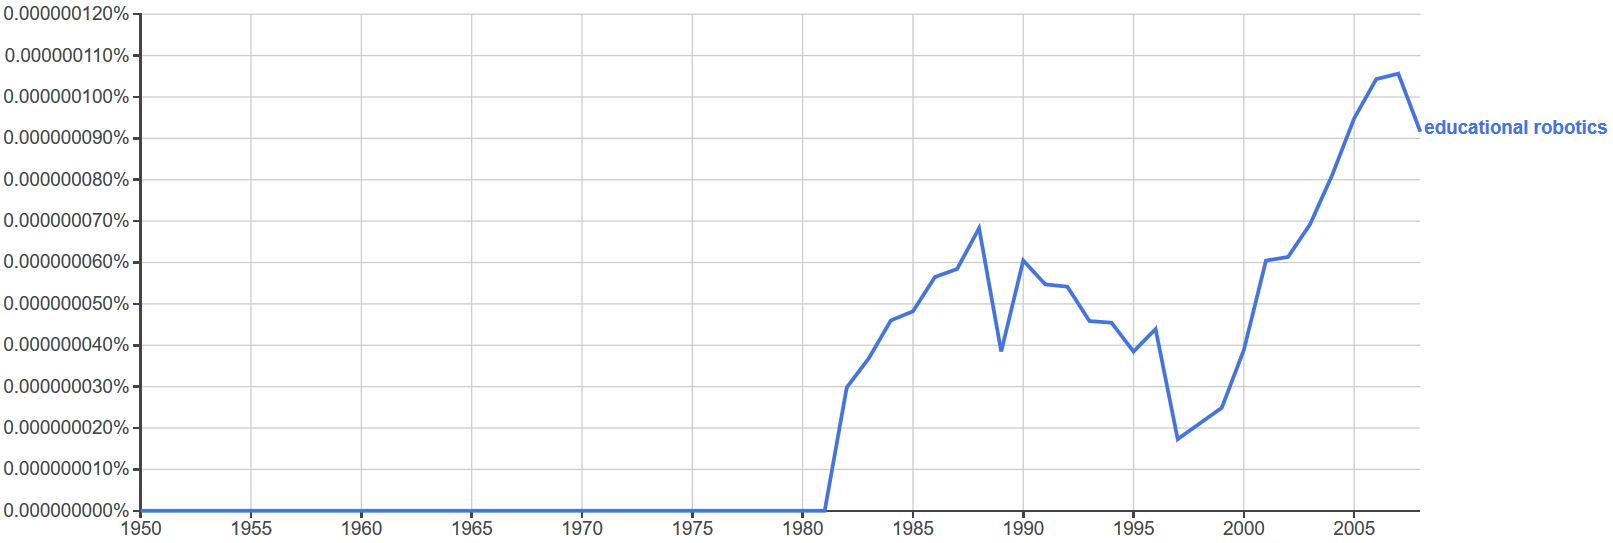
\includegraphics[scale=0.3]{images/ngram.png}
    \caption{Исследование корпуса Google Books English по запросу $[\texttt{educational\ robotics}]$}
    % \label{PO_scheme_img}
\end{figure}


\section*{Облачные технологии}
Автоматизация когнитивных задач в наше время требует значительных вычислительных мощностей, которые не всегда доступны локально. Это требование привело к повсеместному распространению облачных сервисов и <<тонких клиентов>>, позволяющих перенести вычислительно сложные задачи в облако.

Бывшие раньше уделом отдельных специалистов облачные технологии стали доступными любому любознательному энтузиасту --- так или иначе в повседневной деятельности облаками пользуется почти каждый, часто даже не подозревая об этом. Многие также используют облака для решения личных задач, например, для ведения семейного бюджета.

\chapter*{Постановка задачи, рассмотренной в ВКР}
Образовательная робототехника в наши дни набирает популярность, являясь фундаментальным инструментом современных образовательных технологий, требующих постоянного развития.

Робототехнические решения в последнее время получили значительное развитие и стали общедоступными.

Облачные сервисы, позволяющие реализовать как простые, так и самые сложные решения, используя последние достижения компьютерных наук, в последнее время перестали быть сложным малоизвестным инструментом и стали доступны и удобны.

Совокупность вышеприведённых фактов указывает на \textbf{актуальность следующей задачи}: создать и развить средства, позволяющие удобным образом создавать объекты образовательной робототехники, используя передовые технологии.

% \section*{Объект, предмет и цель работы}

В результате проведённого в рамках работы исследования существующих решений, относящихся к поставленной к задаче, популярных и набирающих популярность решений вспомогательных задач и подзадач основной задачи, были окончательно сформулированы объект, предмет и цель работы.

\textbf{Объект работы} --- когнитивный робот как единица образовательной робототехники.

\textbf{Предмет работы} --- реактивно"=делиберативный подход к созданию когнитивных роботов.

\textbf{Цель работы} --- разработка программно"=аппаратного комплекса для создания диалоговых когнитивных роботов на основе реактивно"=делиберативного подхода.

\chapter{Теоретическая часть работы}

\section{Исследование решений, существующих в области объекта работы}

Объектом работы явился когнитивный диалоговый робот как единица образовательной робототехники. Выбор объекта был произведён вследствие исследования существующих единиц образовательной робототехники.

\subsection{Существующие решения в образовательной робототехнике}

Исследование СМИ, сети интернет и центров образовательной робототехники, расположенных в г.\,Москве показало, что сейчас образовательная робототехника состоит в подавляющем большинстве из роботов --- тренажёров для программистов. Представляя наглядную демонстрацию результатов работы программ, эти роботы не несут образовательной нагрузки в смысле осуществления процесса передачи информации --- они выступают в роли инструмента проверки уже усвоенных знаний. 

Популярны также конструкторы, дополненные программируемыми электронными компонентами и, наоборот, электронные компоненты, снабжённые наборами добавляемых внешних механизмов. Такие наборы часто сопровождаются вспомогательной литературой в качестве основного инструмента донесения образовательной нагрузки до конечного обучающегося.

Образовательный процесс как диалог учителя с учеником автоматизирован только в виртуальной среде --- недавно стали появляться чат"=боты и образовательные программы. Популярных, доступных роботизированных решений в реальном мире в сфере образования не существует.

\section{Инструменты, необходимые для роботизации диалога}\label{dialogue-instruments}
В диалоге можно выделить две фундаментальные части, автоматизация которых составит значительную часть автоматизации самого диалога. Во"=первых, так как диалог всегда ведётся на некотором языке, необходим этот самый язык. Во"=вторых, диалог можно рассматривать как последовательность взаимных реакций.

\subsection{Язык в автоматизированном диалоге}\label{language-auto}
Из определения, приведённого в энциклопедии <<Кругосвет>> \cite{lang-krugosvet} следует, что, среди множества факторов определяющих язык, одним из ключевых факторов является цель общения. 

Так как разрабатываемое решение, реализующее помимо прочего инструмент диалога, призвано быть доступным и гибким, конечная цель общения в рамках разработанного решения заранее неизвестна и должна быть определена конечным пользователем решения. Отсюда вытекает необходимость предоставить средства для определения конечного языка конечному пользователю. 





\subsection{Автоматизация реакций}
Диалог можно рассматривать как последовательность реакций, например начало диалога --- это реакция на создание условий, способствующих началу диалога. В процессе диалога ответные реплики являются реакциями на некоторые события, приводящие диалог в некоторое состояние. В процессе диалога можно наблюдать как осмысленные реакции, продиктованные целью общения, так и рефлекторные почти мгновенные реакции на какие"=то события.



\section{Элементы аппаратной платформы роботизированного решения}

Две выделенные в \ref{dialogue-instruments} задачи многократно реализованы программно, поэтому любая аппаратная платформа, обладающая возможностью исполнения программ, написанных на языках общего назначения, сможет так или иначе реализовать роботизацию диалога.  

Как сказано в \ref{popular-instruments}, популярными инструментами доступной робототехники являются микроконтроллеры Arduino и микрокомпьютеры Raspberry Pi. Желание сделать простое в использовании, настройке и сопровождении решение мотивирует ориентировать решение на работу с этими инструментами. 


Подраздел \ref{language-auto} поднял вопрос реализации средств определения языка общения участников диалога. Реализуя связь микроконтроллеров
Arduino и микрокомпьютеров Raspberry Pi, предстоит также реализовать язык взаимодействия этих двух классов устройств, который будет основываться на том или ином средстве передачи данных. Последняя задача требует исследования средств ввода"=вывода, доступных в микроконтроллерах Arduino и микрокомпьютерах Raspberry Pi.

\subsubsection{Средства ввода"=вывода в микроконтроллере Arduino}
Различные продукты семейства Arduino имеют различный набор средств ввода-вывода, гарантированно же присутствуют только ПИНЫ и USB. Популярным дополнительным средством является ethernet.

Плюсы ethernet

Минусы ethernet

Плюсы USB

Минусы USB

Плюсы Пинов

Минусы пинов

\subsubsection{Средства ввода"=вывода в микрокомпьютере Raspberry Pi}
Все продукты семейства Raspberry имеют ПИНЫ, USB, ethernet.

Плюсы ethernet

Минусы ethernet

Плюсы USB

Минусы USB

Плюсы Пинов

Минусы пинов

\section{Подходы к автоматизации диалогов}
Автоматизацию диалога можно рассмотреть как подзадачу искусственного интеллекта. Множество различных идей о решении задач искусственного интеллекта можно разделить на два подхода: \textbf{\textit{подход первый и подход второй}}.

Последний подход основан на моделировании функционирования реальных биологических элементов --- особенно популярным в наши дни примером такого подхода являются нейронные сети. Для решения задачи, поставленной в выпускной квалификационной работе, такой подход кажется мало подходящим потому, что поставленная задача не состоит в моделировании поведения биологических элементов вовсе.

Первый же подход к моделированию интеллектуальных систем, состоящий в нисходящем моделировании высокоуровневых интеллектуальных процессов, кажется подходящим для решения поставленной задачи, состоящей как раз в моделировании высокоуровневого интеллектуального образовательного процесса. Рассмотрим этот подход подробнее.

\subsection{Нисходящий подход в разработке решений искусственного интеллекта}

{\Large Про когнитивность}


\chapter{Практическая часть работы}

Вышеописанные исследования привели к чётко поставленной задаче --- реализовать программно-аппаратный комплекс, который позволял бы максимально доступным образом создавать диалоговых когнитивных роботов. Аппаратная часть комплекса должна быть основана на микроконтроллерах Arduino и микрокомпьютерах Raspberry Pi. Программная часть должна реализовывать логику робота, используя реактивно"=делиберативный подход.

\section{Основные этапы в разработке решения задачи, сформулированной в выпускной квалификационной работе}
Основными этапами разработки явились:
\begin{enumerate}
\item подготовка аппаратной платформы решения 
\begin{itemize}
    \item исследование микроконтроллеров Arduino и микрокомпьютеров Raspberry Pi, представляющих основу аппаратной части, с точки зрения программиста
    \item разработка единой аппаратной платформы, объединяющей Arduino и Raspberry Pi в единый элемент, реализующий поставленную задачу
\end{itemize}

\item разработка необходимого программного обеспечения
\begin{itemize}
    \item выбор технологий для построения программного решения поставленной задачи
    \item выделение ключевых подзадач поставленной задачи в самостоятельные единицы, подлежащие разработке
    \item разработка выделенных на предыдущем этапе элементов
\end{itemize}

\item отладка разработанного решения
\begin{itemize}
    \item отладка разработанного решения
\end{itemize}

\item доработка решения с учётом требований потенциальных пользователей
\begin{itemize}
    \item анализ разработанного решения потенциальными пользователями
    \item доработка разработанного решения с учётом требований потенциальных пользователей
\end{itemize}

\item применение разработанного решения к реальной задаче  
\begin{itemize}
    \item реализация пробного проекта вместе с потенциальными пользователями решения
    \item получение обратной связи от потенциальных пользователей разработанного решения и сторонних компетентных специалистов
\end{itemize}

\item публикация законченного разработанного решения как готового
\begin{itemize}
    \item внедрение разработанного решения в технологический стек потенциальных пользователей решения
    \item публикация исходного кода разработанного решения
\end{itemize}
\end{enumerate}

Этапы разработки подробно раскрыты ниже.

\section{подготовка аппаратной платформы решения}
бла бла

\section{разработка необходимого программного обеспечения}
бла бла
\section{отладка разработанного решения}
бла бла
\section{доработка решения с учётом требований потенциальных пользователей}
бла бла
\section{применение разработанного решения к реальной задаче}
бла бла
\section{публикация законченного разработанного решения как готового}
бла бла

\section{Обоснование принципов действия разработанных объектов}
\subsection{Архитектура разработанного решения}

\section{Характеристики разработанных объектов}

\chapter{Результаты работы}
\section{Обобщение результатов работы}
В работе был рассмотрен и исследован реактивно"=делиберативный подход к созданию когнитивных роботов. Практическим результатом работы является разработанный программно"=аппаратный комплекс для создания диалоговых когнитивных роботов на основе реактивно"=делиберативного подхода. 

Разработанный программно"=аппаратный комплекс был использован в когнитивных диалоговых роботах <<Подушка>> компании МеханиУм. Роботы были представлены на мероприятиях Российский финал Microsoft Imagine Cup 2018, Skolkovo Robotics Forum 2018. Один из роботов <<Подушка>> стал экспонатом музея <<Открытый космос>>. 
\section{Оценка результатов работы}
\subsection{Оценка полноты решения поставленной задачи}

\chapter{Заключение}
\section{Положения, выносимые на защиту}
\subsection{Общие результаты работы}
\subsection{Выводы, сделанные в процессе работы}
\subsection{Предположения, сделанные в процессе работы}
\section{Дальнейшее развитие}
\subsection[Перспективы применения результатов работы \\на практике]{Перспективы применения результатов работы на практике}
\subsection{Возможности дальнейшего исследования проблемы}
\end{document} 
